\chapter{Implementation}

\todo{Introduction to chapter : - Analysis of the Data - Methods developed - Algorithm Implementation - Results Analysis (viz and comparison) }

\section{Data Analysis}

As the main dataset, we use the simulation results on an unstructured mesh of measurements with a very high density in the low middle part of the space. The simulation used has $100'040$ points over $988$ timestamps. 


 Several fields are present in the simulation : the \textbf{pressure}, the \textbf{tracer} concentration, the \textbf{background tracer} concentration and the \textbf{velocity}. \\ 

The \textbf{tracer} represents the propagation of a pollutant generated from the centre of the domain at ground level. It aims a representing a busy intersection. We represent two horizontal cuts of the tracer field at $z=1m$ and at $t=50$ and $t=988$ in the figures \ref{fig:view:tracerstart} and \ref{fig:view:tracerend}\\


\begin{figure}[h!]
\centering
  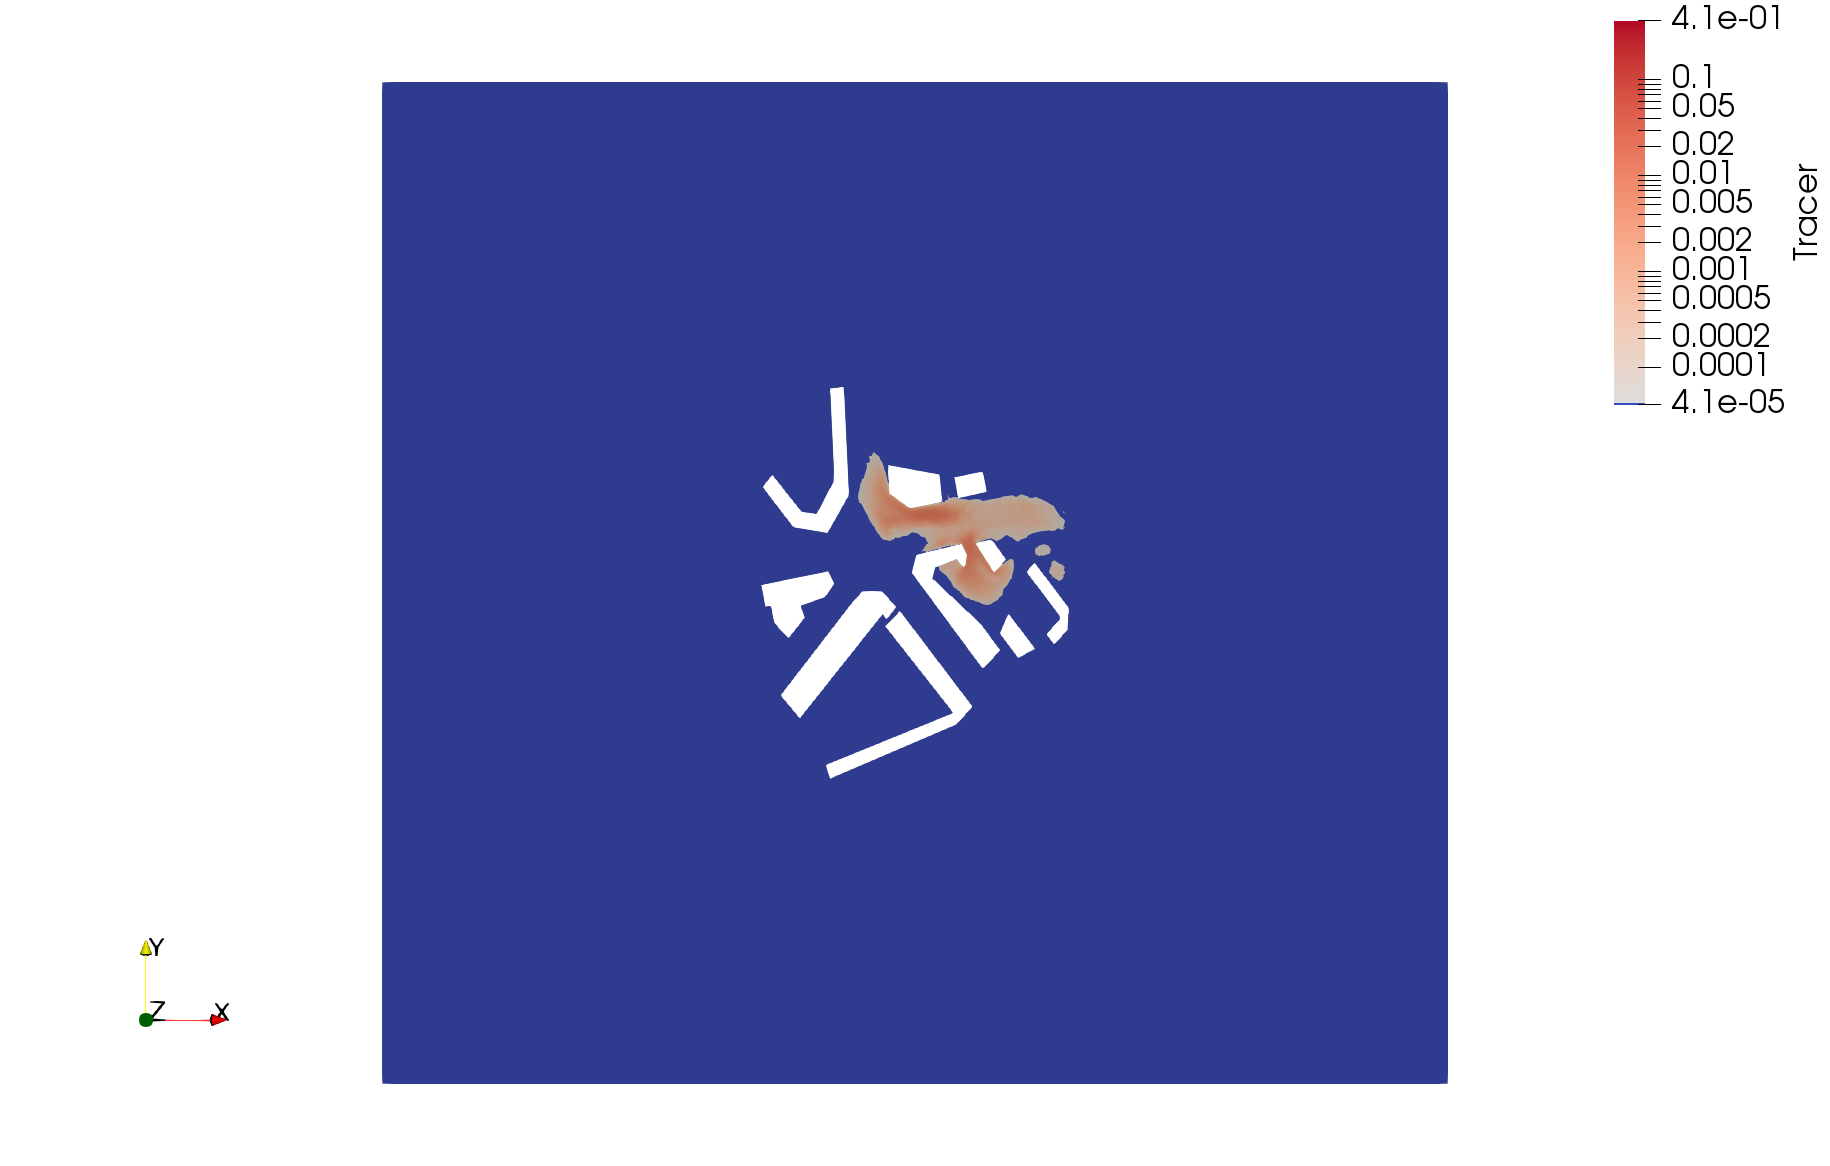
\includegraphics[width=0.9\linewidth]{figures/Analysis/tracer050cutZ1}
  \caption{Tracer Field : Horizontal cut at $z=1m$ and $t=50$  }
  \label{fig:view:tracerstart}
\end{figure}

\begin{figure}[h!]
\centering
  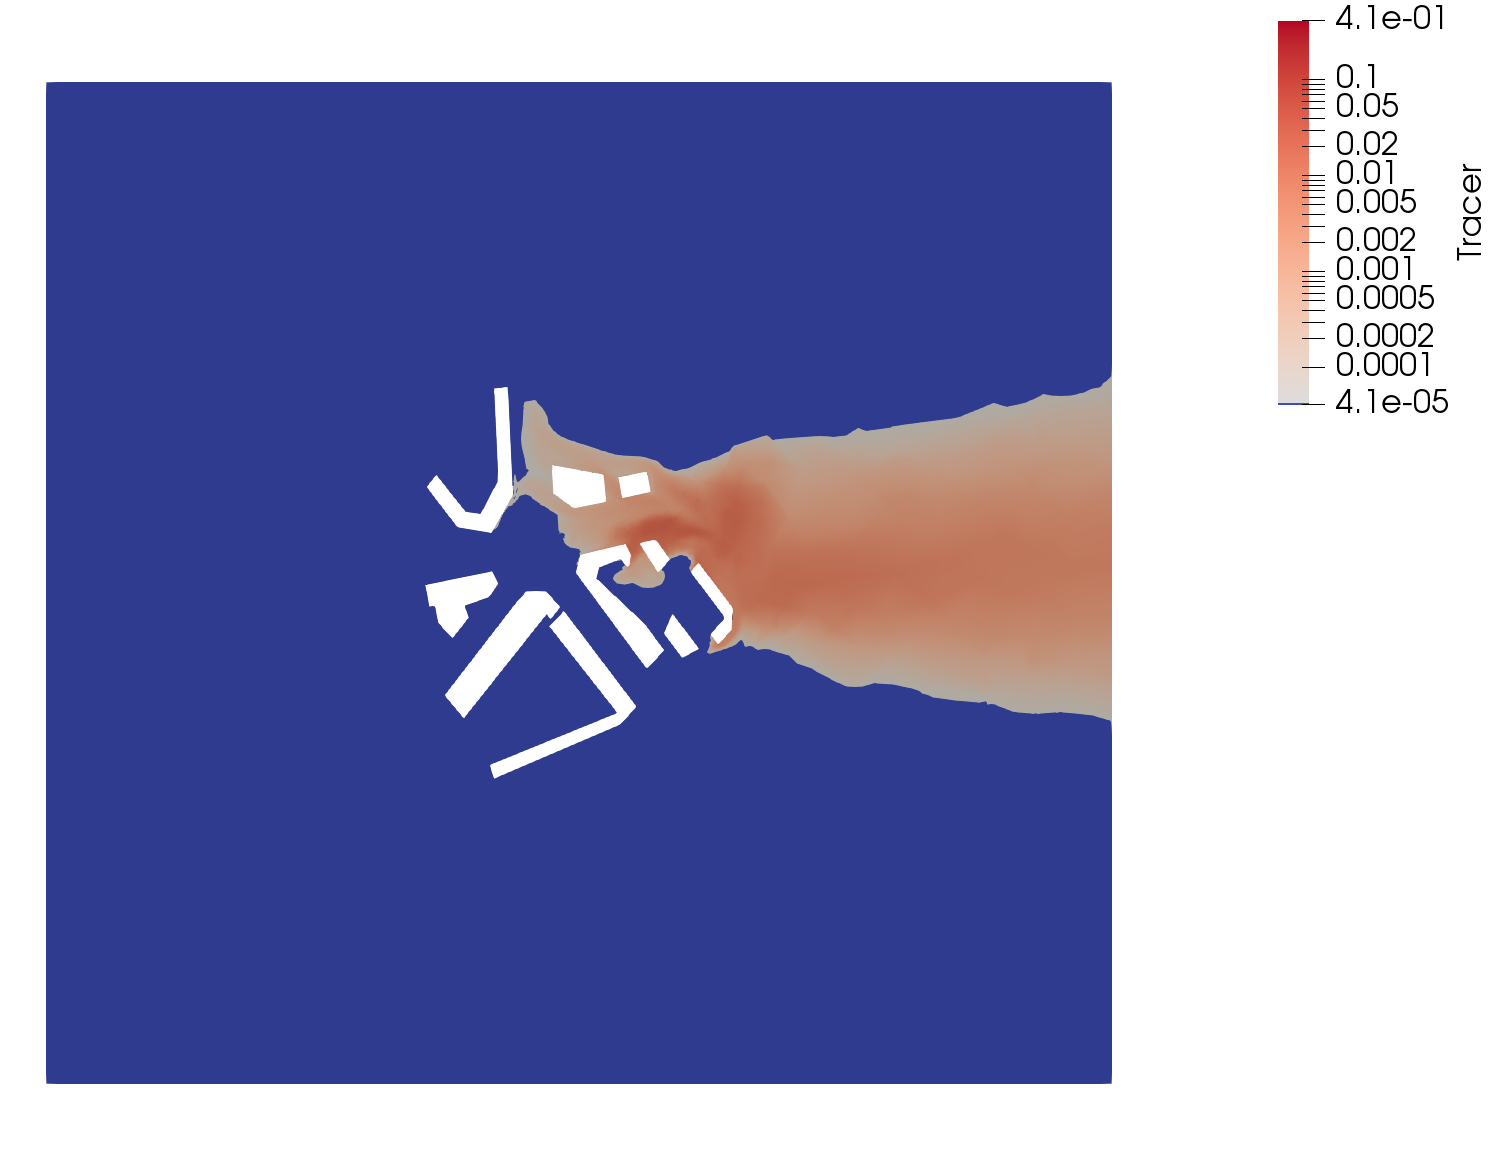
\includegraphics[width=0.9\linewidth]{figures/Analysis/tracer988cutZ1}
  \caption{Tracer Field : Horizontal cut at $z=1m$ and $t=988$}
  \label{fig:view:tracerend}
\end{figure}



As we can see by observing the time propagation of those fields,  the wind is pushing the pollutants in a certain direction. Because of this, be observe that the \textbf{tracer} concentration is mainly visible downwind, in contrast of the \textbf{background tracer} which has visible propagation over the whole space. We can therefore already deduce that the \textbf{background tracer} contains much more information and should be used for optimising the sensor positions. 



\todo{define somewhere the metric we use to see how close are the datasets}

\section{Preselection of the Data} \label{sec:preselection}

For the purpose of testing our codes and algorithms,  we are going to use a subset of the whole dataset containing a few hundreds to a few thousands of points. 

\todo{rewrite the introduction of this section}

The raw data is contained in VTK files. I have implemented functions in python that allows the importation, the cropping of the space, the extraction of the fields and interest and the location of the points and the saving in files for making quicker the loading procedure. 

\subsection{Selection of a working subset of the data}
The first approach that we have in order to reduce the number of the potential sensor locations, is the reduction of the space in which  we run our optimisation problem. We are focusing on the \textit{tracer} field of the simulation data. This field contains the propagation of a pollutant originating at the \textbf{center of the space} and under wind conditions blowing in the \textit{east direction} (see figure \ref{fig:view:tracer} ). The resulting data shows that most of the space is unaffected by this pollutant and so we wish to select only the space in which the pollutant concentration is non negligible. For that we develop the following procedure. \\

First we cut our 3D space into cuboids. For that we fix a number of bins per dimension and we obtained $R$ subsets $\{\mathcal{D}_k\}_{k=0}^R $. For each subspace we compute the sum over time and space of the tracer values $Y_t^i$  : 

\begin{equation}
	C(\mathcal{D}_i) = \sum_{k \in \mathcal{D}_i} \sum_{t = 0}^T Y_t^k
\end{equation}

We apply then a selection of the subsets based on the value of $C(\mathcal{D}_i)$ and a  threshold $\tau$. We keep then every subset $\mathcal{D}_i$ that respects the condition : $C(\mathcal{D}_i) > \tau$. This condition but guarantees that the points kept in the new working subset $S$ have a sufficient importance in the physical world. The new working subset for our optimisation problem would then be : 

\begin{equation}
	S = \bigcup_{C(\mathcal{D}_i) > \tau} \mathcal{D}_i
\end{equation} 

An example of this algorithm is now explained. For a number of bins of 25 in each dimension and threshold of $\tau = 10^{-2}$ we obtain a new working set size $|S| = 57'725$ instead of an original number of $100'040$. It is displayed on the figure \ref{fig:working_subset}


\begin{figure}[h]
\centering
	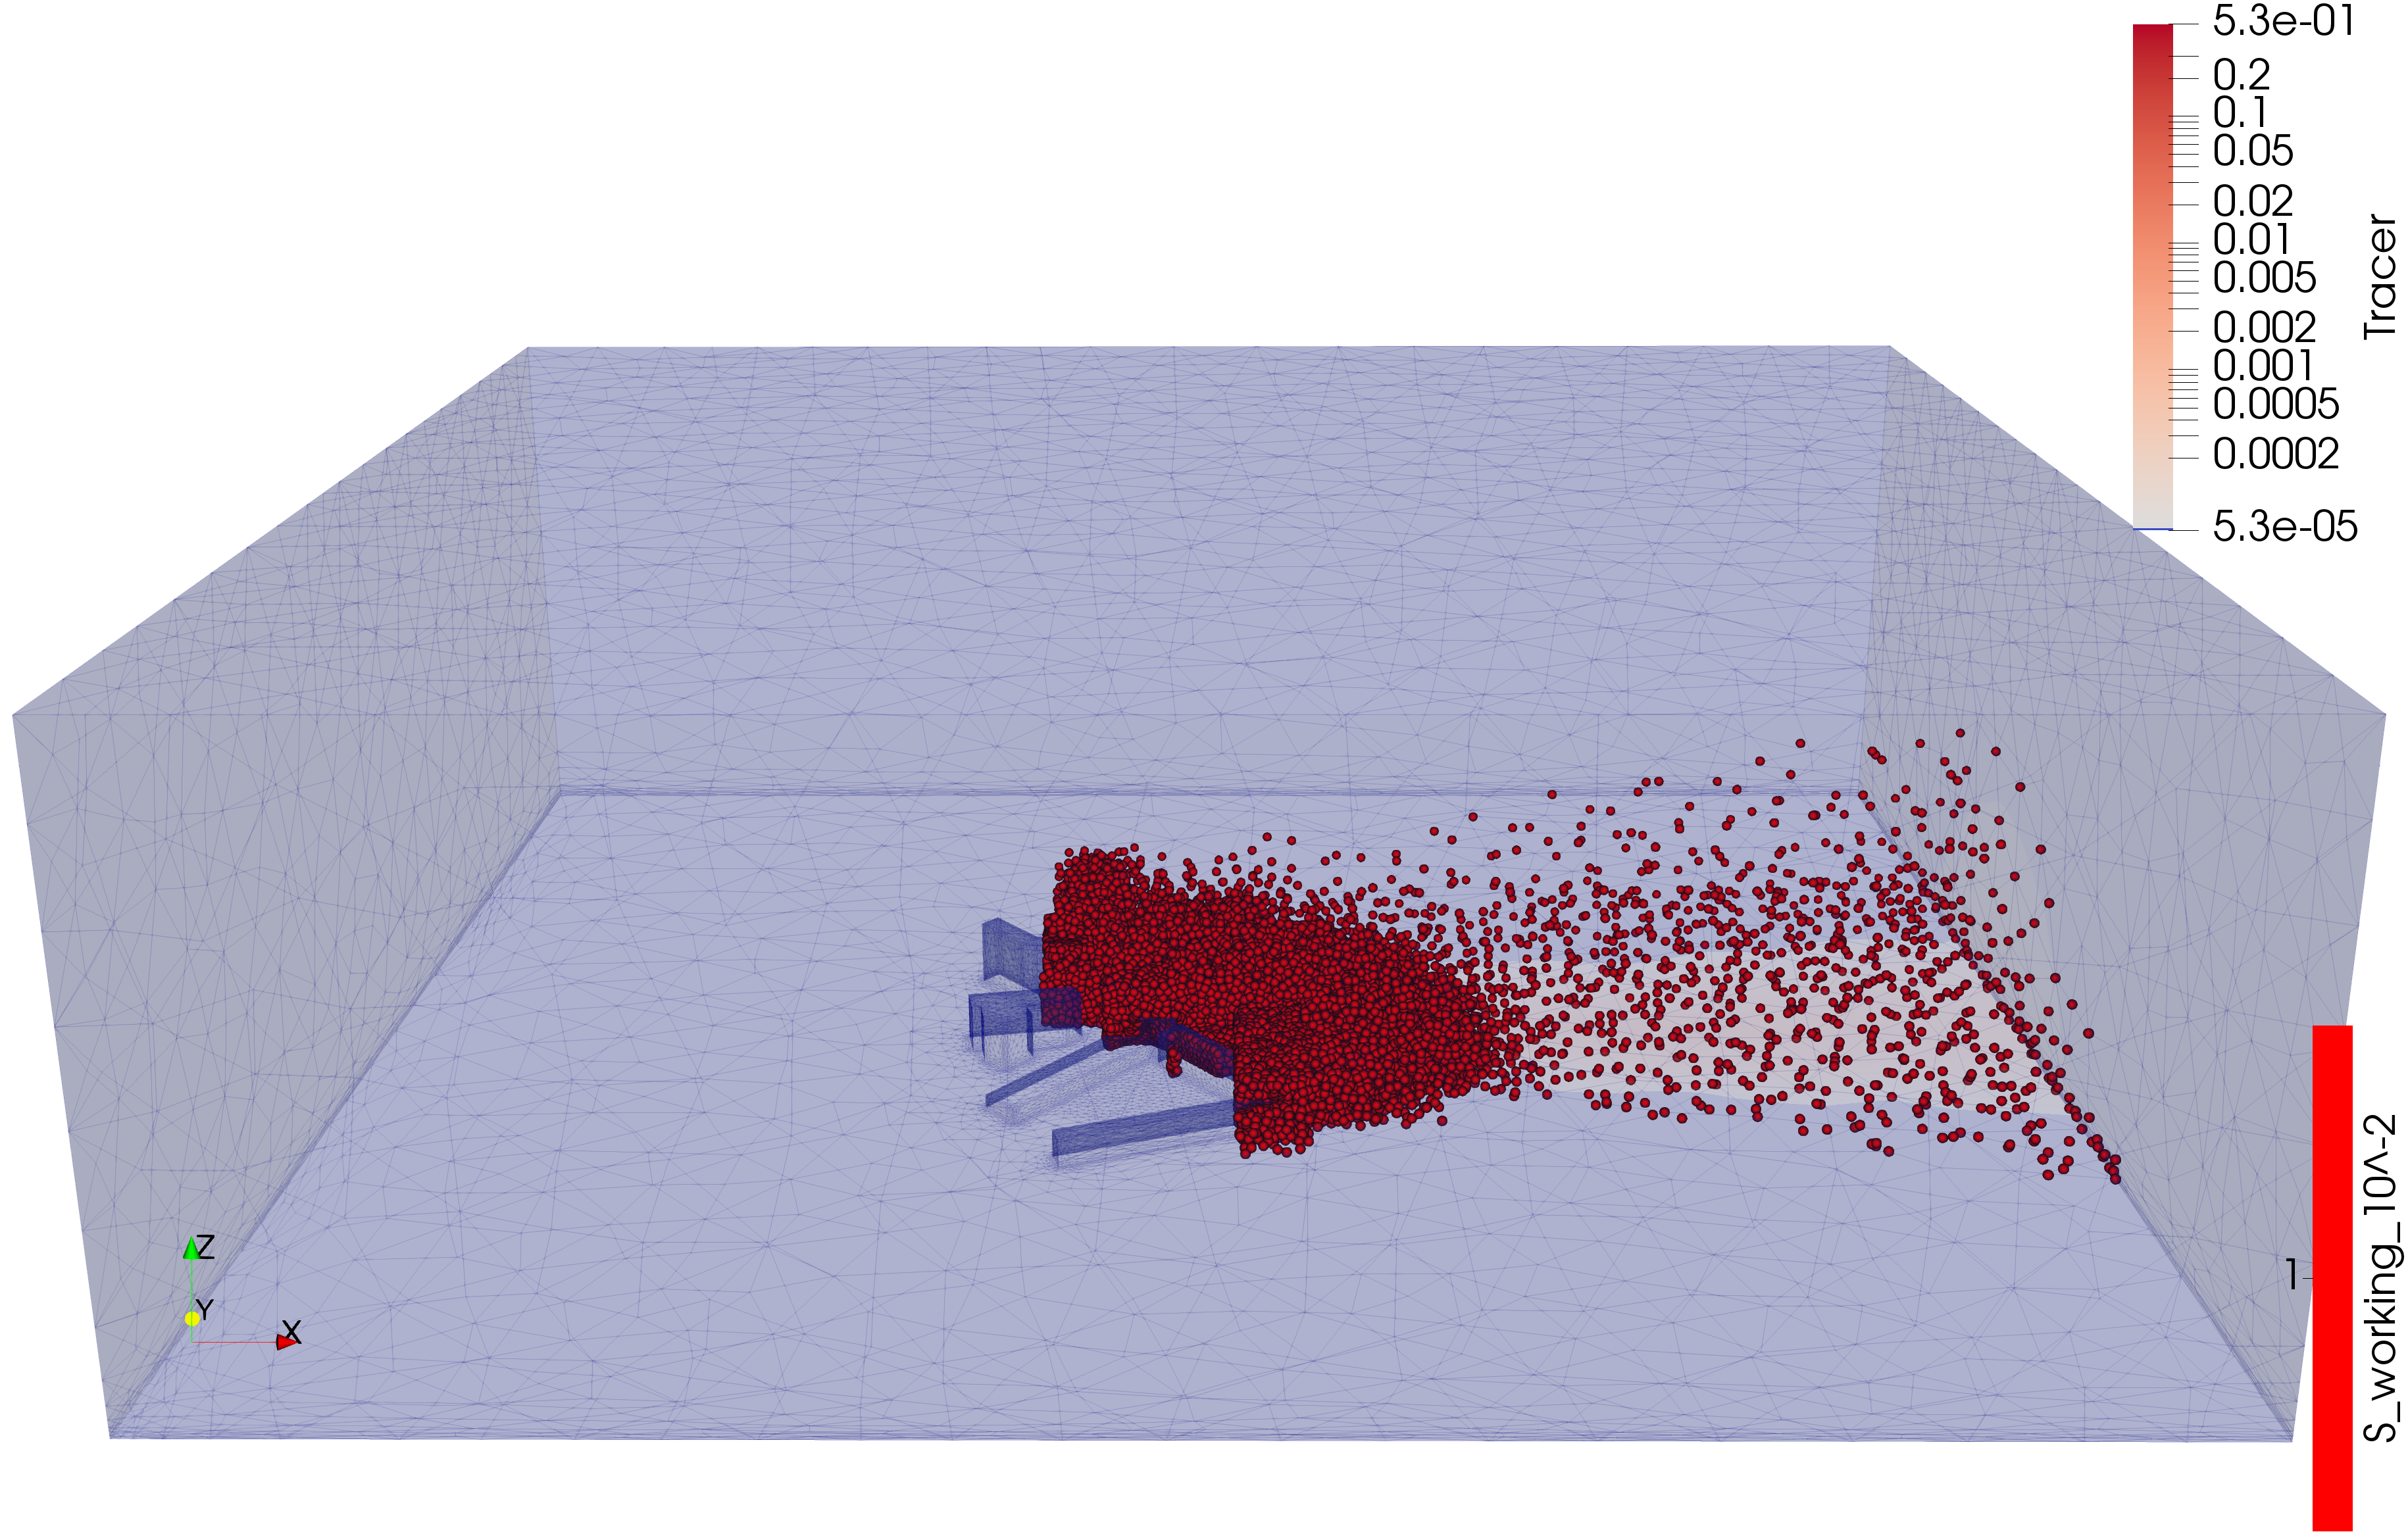
\includegraphics[width = 0.8 \textwidth]{figures/Subset/working_subset_10^-2}
	\caption{New working subset $S$ for $\tau = 10^{-2}$}
	\label{fig:working_subset}
\end{figure}

\subsection{Selection of a subset at human level}

In order to further reduce the number of points involved in the optimisation problem, we can also consider taking points that are only accessible by a human from the ground level or the buildings. This makes sense in the way that sensors needs to be reached from the ground and the  building top and sides for their initial placement and maintenance. We define for each building $i \in \{1, \dots, B\}$ an altitude $H_i$, and for $i = 0$ we consider the rest of the unoccupied space, so $H_0 = 0$. This allows us to define an altitude under which we will select the points : $H_i + h$. The area covered by the buildings is enlarged by the value $w$, so that is covers also the sides of the buildings. See the illustration provided in figure \ref{fig:humanchart}. \\

\begin{figure}[h]
\centering
	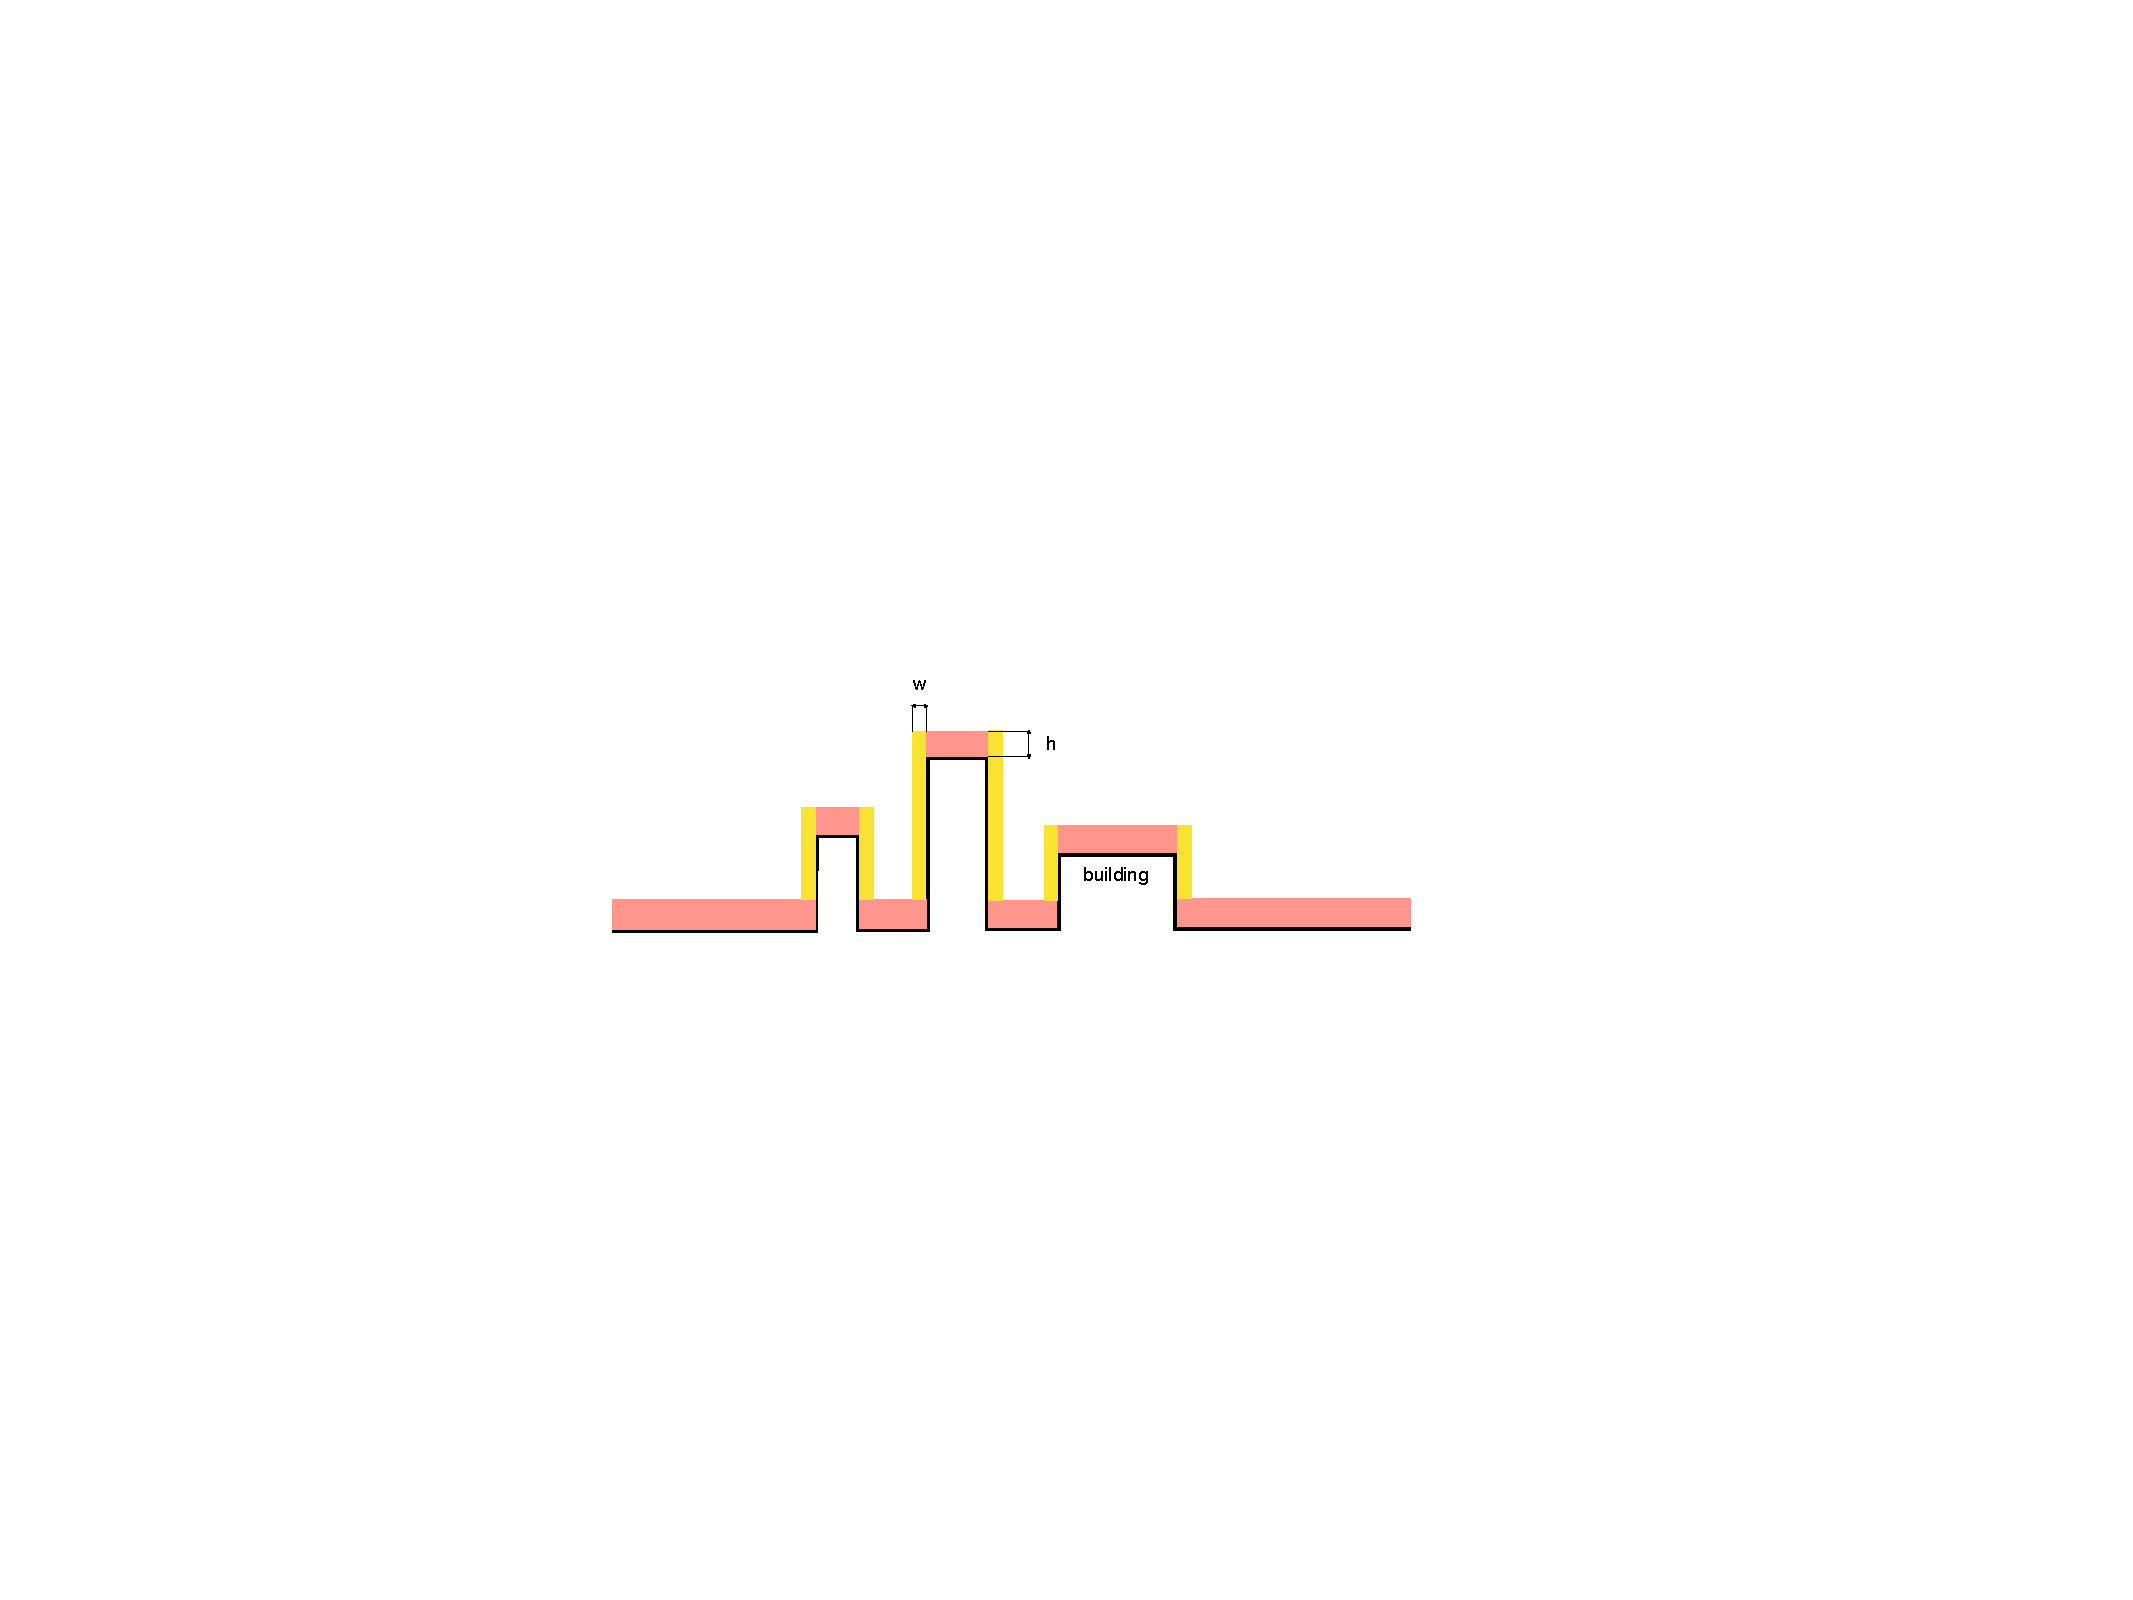
\includegraphics[width = 0.6 \textwidth]{figures/Subset/HumanSelection_chart}
	\caption{Chart Presenting the Building Profile in Human Level Selection}
	\label{fig:humanchart}
\end{figure}

In order to proceed to this selection, I had to overcome the absence of defined building profile and I had to manually define the shapes of the buildings (as you can see on figure \ref{fig:buildingshapes}) by taking the empirically the coordinates of the buildings in the small LSBU dataset, considering a XY projection of the 3D space. \\

\begin{figure}[h]
\centering
	
\includegraphics[width = 0.25 \textwidth]{figures/Subset/buildingShapes_13}
	\caption{Empirical Building Shapes}
	\label{fig:buildingshapes}
\end{figure}

\todo{make ref to shapely}
Once those coordinates acquired, I used the shapely package in order to define the polygones associated to the buildings. In order to define the height $H_i$ of each building I had to define a set of points overhanging it and find the minimal altitude of this point.  To define the set of points I took the inner part of the surface of the building (cut by 1m) in order to avoid any edge point. This can be seen on the figure \ref{fig:inner_outer_building}). The points which have XY coordinates within this shape are then selected and the minimal Z coordinate is taken as the definition of the roof level $H_i$ \\


\begin{figure}[h]
\centering
	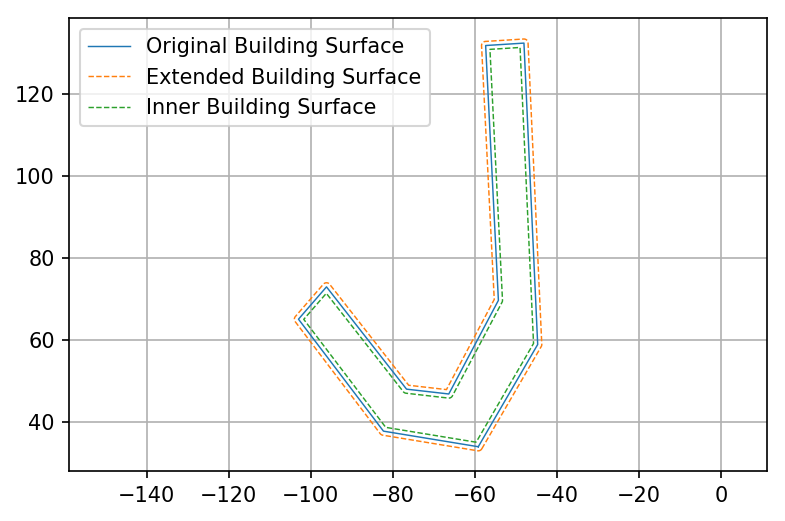
\includegraphics[width = 0.7 \textwidth]{figures/Subset/BuildingSurfaceBuffer}
	\caption{Extended an Inner building surface}
	\label{fig:inner_outer_building}
\end{figure}

Once the roof level defined we come back to the original shape of the building and enlarge it of $w$ such as showed in figure \ref{fig:inner_outer_building}. We then select every point of the main dataset that have XY coordinates in this extended rooftop and   choose only the ones which have Z bellow the threshold $H_i + h$. This constitutes our human level data selection. An illustration can be found on figure 

\begin{figure}[h!]
\centering
	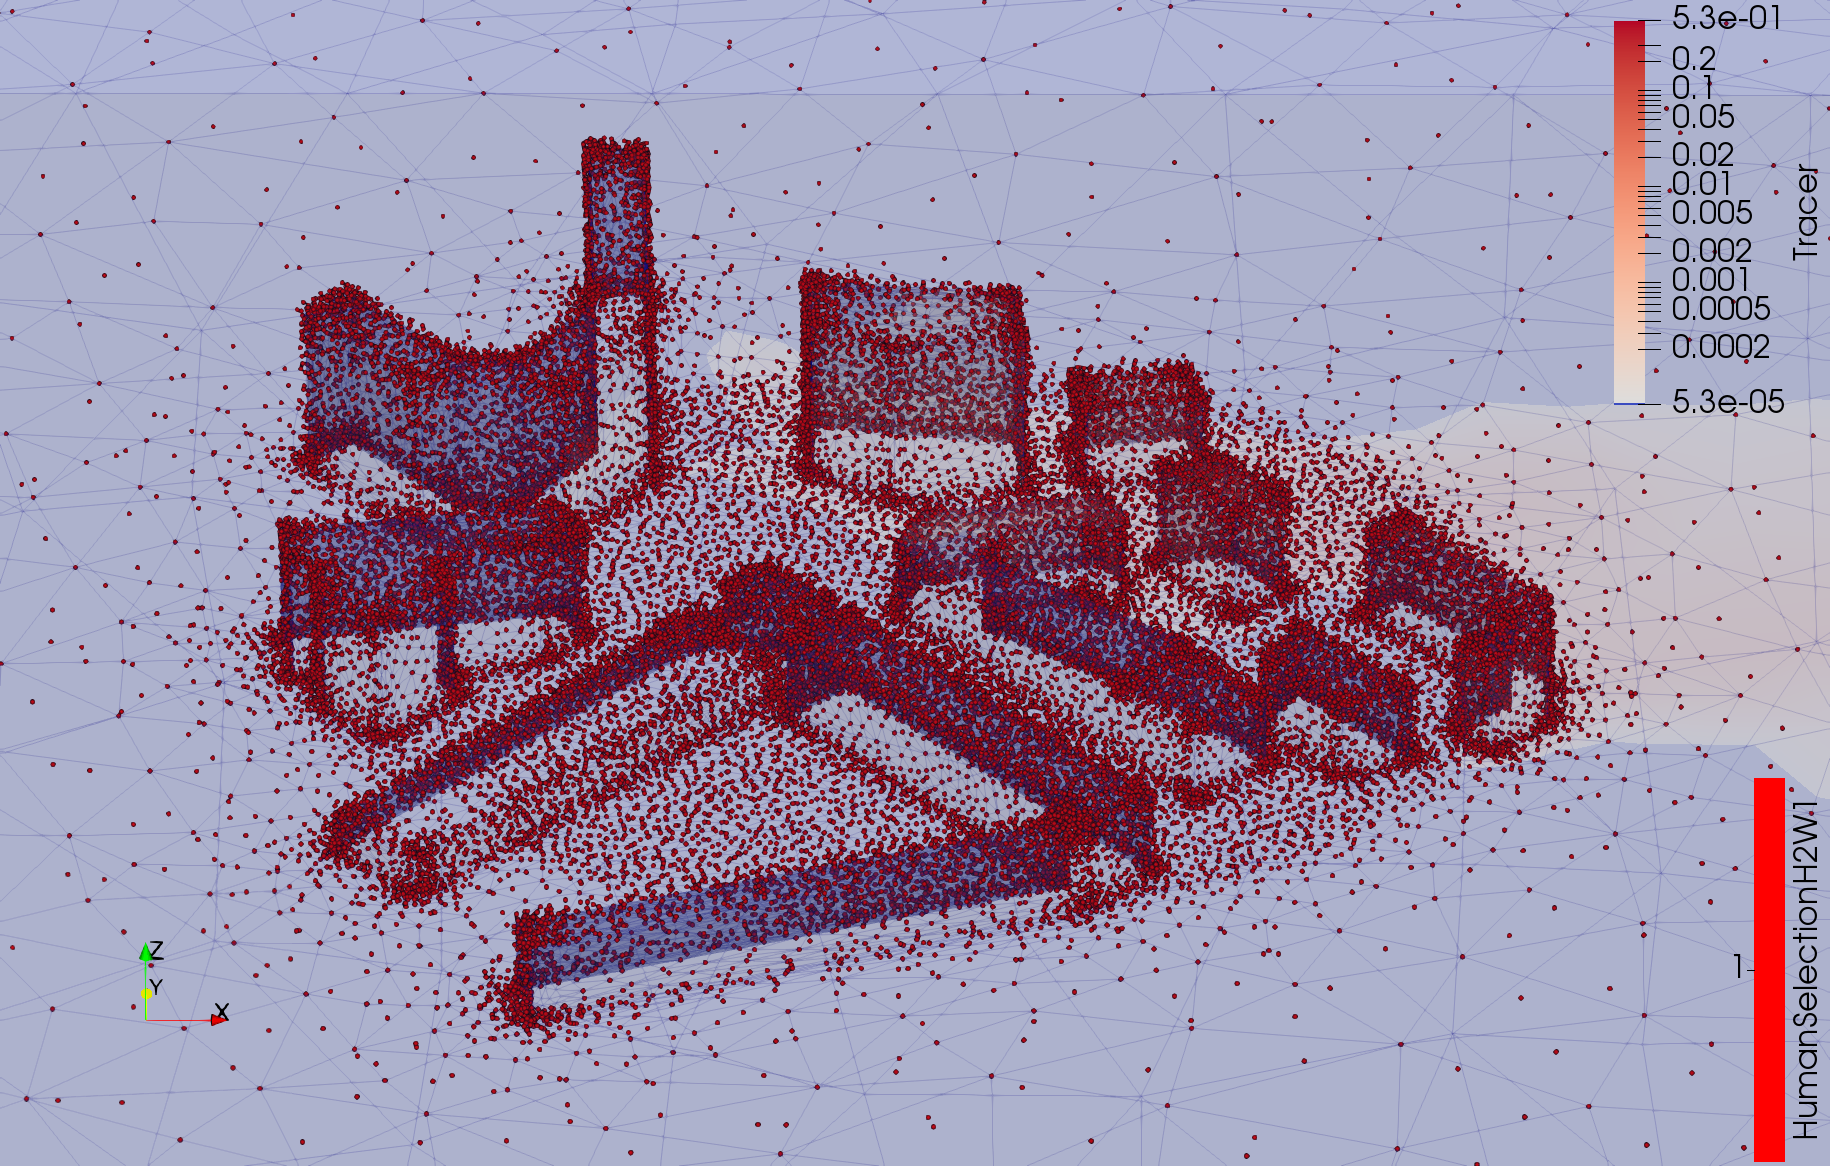
\includegraphics[width = 0.8 \linewidth]{figures/Subset/HumanSelectionH2W1_zoom}
	\caption{Human Level Selection}
	\label{fig:human_selection}
\end{figure}

This method can be seen as quite empirical, but it enables a precise dataset selection with no outlying point. The other approaches were not giving such good results. \\

With the parameters $h = 2m$ and $w = 1m$ we reduce the size of the dataset to $|S| = 37'847$. 


\subsection{Combined Selection}

By combining the two selection approaches and by taking the intersection of the two previously defined datasets : the working subset based on the values of the tracer and the human level selection. We are able to reduce the number of points in the dataset to $|S| = 23'643$, instead of an original number of $100'040$, which is a reduction of $76.36\%$ of the original size. In the figure \ref{fig:combined_selection} we see an illustration of the selected dataset that will be used in the rest of the project. 

\begin{figure}[h!]
\centering
	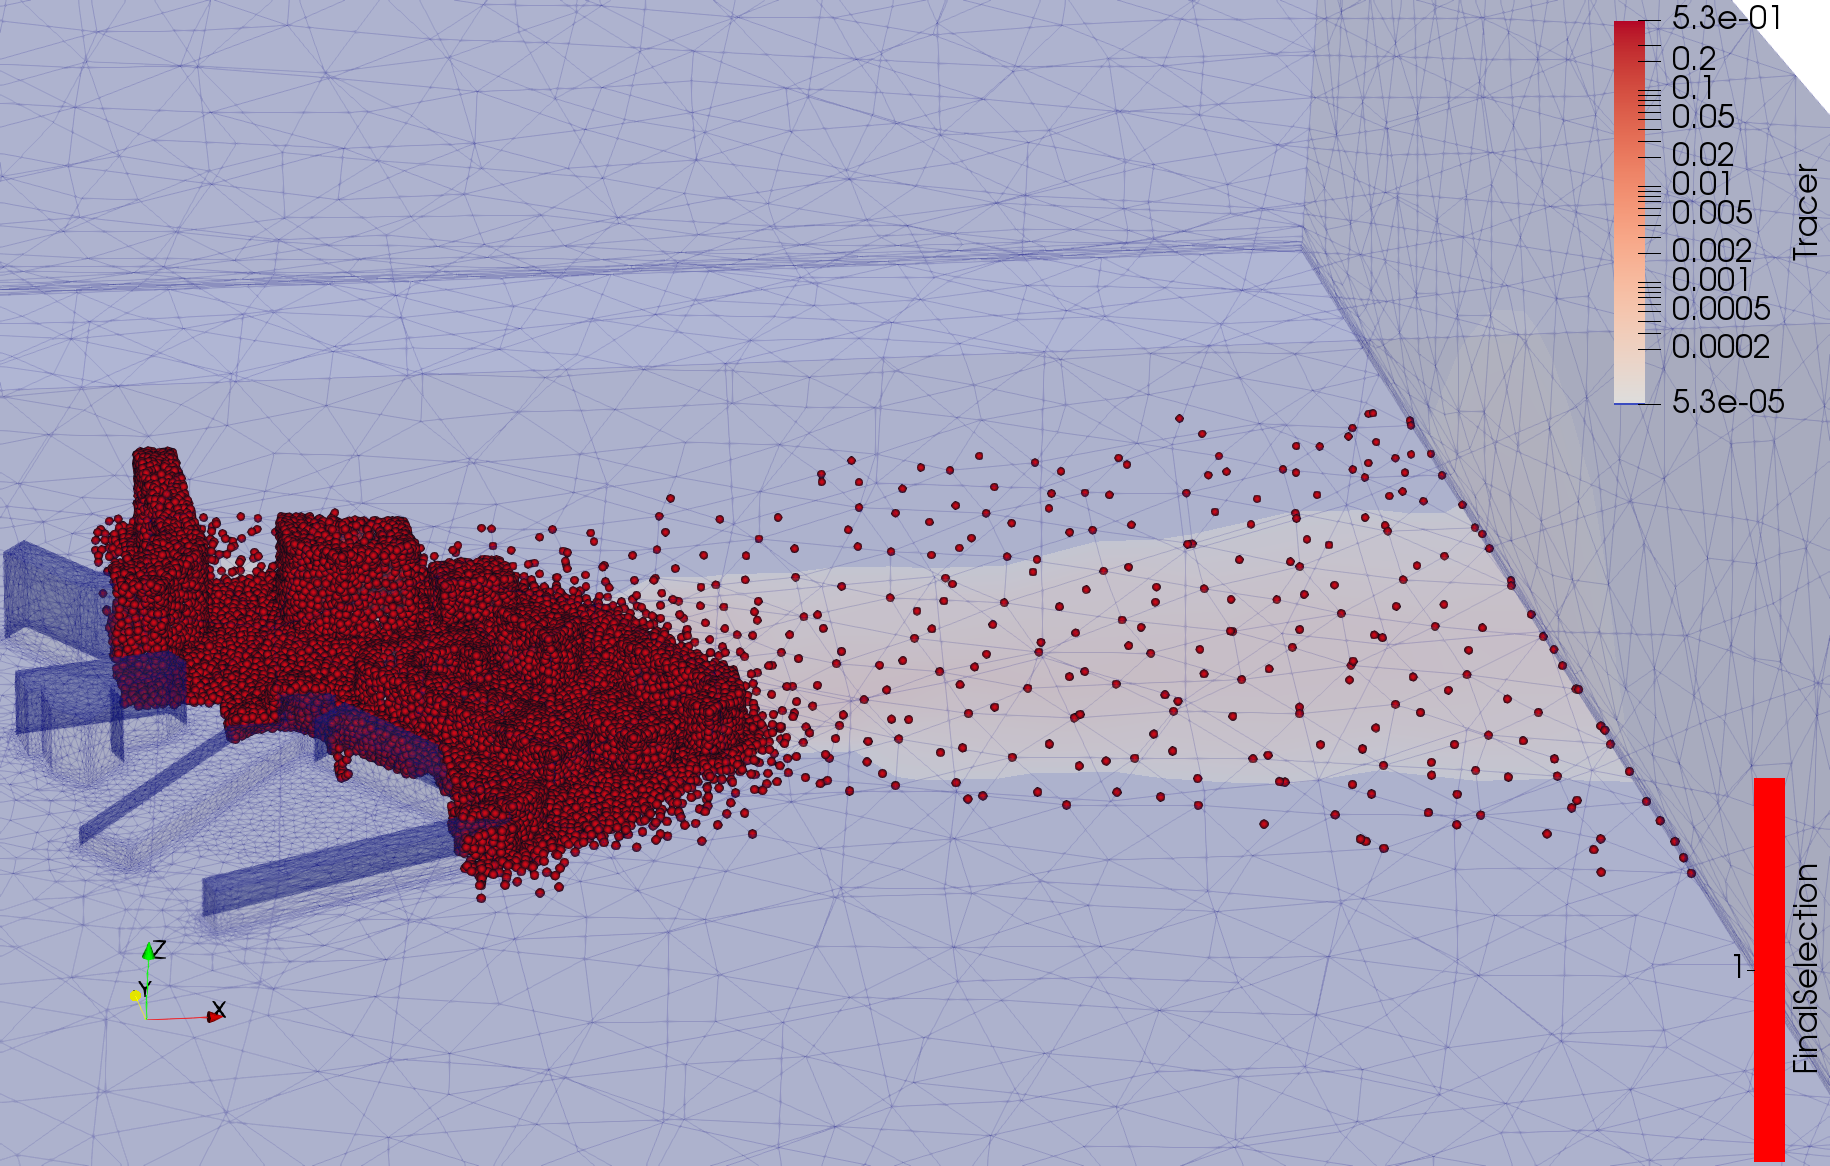
\includegraphics[width = 0.8 \linewidth]{figures/Subset/FinalSelection_zoom}
	\caption{Combined Selection : Working Subset and Human Level Selection}
	\label{fig:combined_selection}
\end{figure}
 


\section{Implementation of the Gaussian Process}

\todo{Important to explain how the gaussian processes were implemented. Challenge of the inversion. Classical approach and TSVD approach and show simple computation times and error results.} 

\subsection{Classical Gaussian Process}

\subsection{Approximation Gaussian Process}

In to reduce the computational cost of the Gaussian Process, we proposed a method that allows 

\section{Implementation of the Optimisation Algorithm}


\todo{Explain every algorithm implemented, their difference. This is important for the result section where sample results for those algorithm will be shown later on }


\section{Implementation of Variational Data Assimilation}

\todo{Write this in the end only if the validation works well}



